\documentclass[../notes.tex]{subfiles}
\graphicspath{{\subfix{../images/}}, {\subfix{../}}}

\begin{document}

\chapter{Superconductivity}

In 1894, Albert Michelson remarked that \enquote{it seems probable that most of the grand underlying principles have been firmly established} \cite[p. 159]{chicagoAnnualRegister1896}.


At the end of the 19th and the beginning of the 20th century, cooling technology made great progress.
Liquifying gases, were able to reach temperatures as low as \(\qty{4}{\kelvin}\) (the boiling point of Helium).
Using that, SC was discovered in mercury in 1911 by Heike Onnes \cite{onnesFurtherExperimentsLiquid1991}.
Superconductivity describes the phenomenon of the electrical resistance of a material suddenly dropping to zero below a critical temperature \(T_C\).
Discovery of Meissner effect, perfect expulsion of external magnetic fields in 1933 \cite{meissnerNeuerEffektBei1933}.
This started almost half a century of intensive theoretical research, which culminated in John Bardeen, Leon Cooper and J. Robert Schrieffer developing the microscopic theory now know as BCS theory \cite{bardeenTheorySuperconductivity1957}.
1986 and 1987: discovery of superconductivity with very high \(T_C\) found in cuprates \cite{bednorzPossibleHighTc1986,uchidaHighTcSuperconductivity1987}.
Cuprate superconductors are made up of layers of cooper oxide and charge reservoirs in between.
The specific charge reservoir layers determine the properties of the SC and varying them lead to a rich zoo of materials with high \(T_C\)  \cite{rybickiPerspectivePhaseDiagram2016}.

Largest commercial application to date is in magnetic resonance imaging, a medical technique using strong magnetic fields and field gradients \cite{rinckMagneticResonanceMedicine}.
Enabled due to the fact, that SCs can carry much stronger currents and thus generate much higher magnetic field strength.
Technical applications in research are much wider, ranging from strong superconducting magnets in the LHC \cite{tollestrupDevelopmentSuperconductingMagnets2008} and other particle accelerators over detectors of single photons in astrophysics \cite{irwinTransitionEdgeSensors2005} to extremely sensitive measurement devices for magnetic fields \cite{faleyHighTcSQUIDBiomagnetometers2017} and voltages \cite{klushinPresentFutureHightemperature2020} based on the Josesphon effect \cite{josephsonPossibleNewEffects1962}.


Since the first discovery of SC in cuprates, there has been a lot of work to develop superconductors with higher transition temperatures.
One interesting development in is in twisted multilayer systems, first realized as twisted bilayer Graphene \cite{caoUnconventionalSuperconductivityMagicangle2018}.
In comparison to the complex crystal structure of e.g. the Cuprates, twisted multilayer systems have a very simple structure and can be tuned very easily: the angle of twist between the layers can be easily accessed experimentally.
The defining feature of these systems are flat electronic bands due to folding of the Brilluoin zone.
Superconductivity in these systems is enhanced due to the fact that in the flat bands, interactions between the electrons are very strongly enhanced.
Thus these systems are a very interesting playground to study strongly correlation effects in general and superconductivity in particular.

This chapter: introduction to the mean-field BCS theory in \cref{sec:bcs-theory}, GL-theory in \cref{sec:Ginzburg-Landau theory of superconductivity} and


\section{Ginzburg-Landau Theory of Superconductivity}\label{sec:Ginzburg-Landau theory of superconductivity}

Following~\cite[ch. 11]{colemanIntroductionManyBodyPhysics2015}.

\paragraph{Order parameter}

Landau theory: phase transitions (e.g.\ iron becomes magnetic, water freezes, superfluidity/superconductivity) are associated with the development of an order parameter when the temperature drops below the transition temperature \(T_C\).
\begin{equation}
	\vert \psi \vert =
	\begin{cases}
		0\;,\; T > T_C \\
		\vert \psi_0 \vert > 0 \;,\; T < T_C
	\end{cases}
\end{equation}
Landau theory does not need microscopic expression for order parameter, it provides corse-grained description of the properties of matter.
The order parameter description is good at length scales above \(\xi_0\), the coherence length (e.g.\ size of Cooper pairs for SC).
On length scales above \(\xi_0\), the order parameter behaves as a smoothly varying function.

\paragraph{Landau theory}

Basic idea of Landau theory: write free energy as function \(F[\psi]\) of the order parameter.
Region of small \(\psi\), expand free energy of many-body system as simple polynomial:
\begin{equation}
	f_{L} = \frac{1}{V} F[\psi] = \frac{r}{2} \psi^2 + \frac{u}{4} \psi^4
\end{equation}
Provided \(r\) and \(u\) are greater that \(0\): minimum of \(f_L [\psi])\) lies at \(\psi = 0\).
Landau theory assumes: at phase transition temperature \(r\) changes sign, so:
\begin{equation}
	r = a(T - T_C)
\end{equation}
Minimum of free energy occurs for:
\begin{equation}
	\psi = \begin{cases}
		0 \\
		\pm \sqrt{\frac{a (T_C - T)}{u} }
	\end{cases}
\end{equation}

Two minima for free energy function for \(T < T_C\).
With this, we can extract \(T_C\) from the knowledge of the dependence of \(\vert \psi \vert^2\) on \(T\) via a linear fit.
This is only valid for an area near \(T_C\) (where Landau theory holds), but can be used to get \(T_C\) from microscopic theories.

Going from a one to a \(n\)-component order parameters, OP acquires directions and magnitude.
Particularly important example: complex or two component order parameter in superfluids and superconductors:
\begin{equation}
	\psi = \psi_1 + \iu \psi_2 = \vert \psi \vert e^{\iu \phi}
\end{equation}
The Landau free energy takes the form:
\begin{equation}
	f[\psi] = r(\psi^* \psi) + \frac{u}{2} (\psi^* \psi)^2
\end{equation}
As before:
\begin{equation}
	r = a(T - T_C)
\end{equation}

Figure~\ref{fig:Landau free energy mexican hat potential} shows the Landau free energy as function of \(\psi\).

\begin{figure}[t]
	\centering
	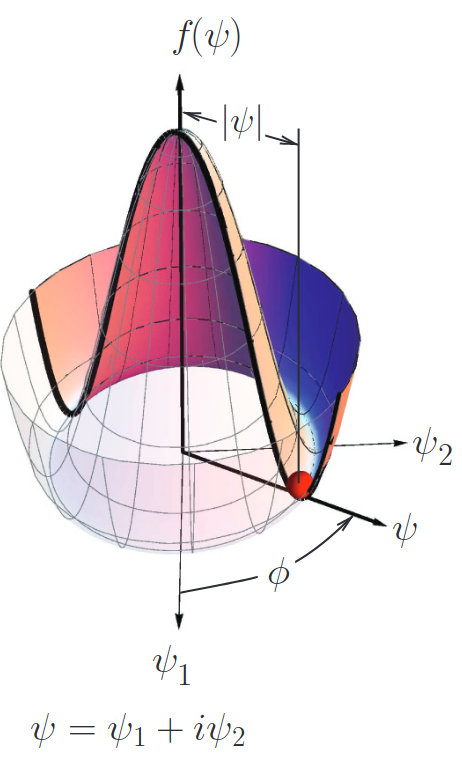
\includegraphics[width=0.3\textwidth]{images/landau free energy mexican hat}
	\caption{Mexican hat potential}
	\label{fig:Landau free energy mexican hat potential}
\end{figure}

Rotational symmetry, because free energy is independent of the global phase of the OP:
\begin{equation}
	f [\psi] = f [e^{\iu a } \psi]
\end{equation}
In this `Mexican hat' potential: order parameter can be rotated continuously from one broken-symmetry state to another.
If we want the phase to be rigid, we need to introduce an
There is a topological argument for the fact that the phase is rigid.
This leads to Ginzburg-Landau theory.
Will see later: well-defined phase is associated with persistent currents or superflow.

\paragraph{Ginzburg-Landau theory}

Landau theory: energy cost of a uniform order parameter, more general theory needs to account for inhomogenous order parameters, in which the amplitude varies or direction of order parameter is twisted -> GL theory.
First: one-component, `Ising' order parameter.
GL introduces additional energy \(\delta f \propto \vert \Delta \psi \vert^2\), \(f_{GL} [\psi, \Delta \psi] = \frac{s}{2} \vert \Delta \psi \vert^2 + f_L [\psi(s)]\), or in full:
\begin{equation}
	f_{GL} [\psi, \Delta \psi, h] = \frac{s}{2} (\Delta \psi)^2 + \frac{r}{2} \psi^2 + \frac{u}{4} \psi^4
\end{equation}
GL theory is only valid near critical point, where OP is small enough to permit leading-order expansion.
Dimensional analysis shows: \(\frac{s}{r} = L^2\) has dimension of length squared.
Length scale introduced by the gradient term: correlation length
\begin{equation}
	\xi (T) = \sqrt{\frac{s}{\vert r(T) \vert}} = \xi_0 \left\vert 1 - \frac{T}{T_C} \right\vert^{-\frac{1}{2}}
\end{equation}
sets characteristic length scale of order-parameter fluctuations, where
\begin{equation}
	\xi_0 = \xi (T = 0) = \sqrt{\frac{s}{\alpha T_C}}
\end{equation}
is a measure of the microscopic coherence length.
Near transition \(\xi (T)\) diverges, but far from transition it becomes comparable with the coherence length.

\paragraph{Complex order and superflow}

Now: GL theory of complex or two-component order parameters, so superfluids and superconductors.
Heart of discussion: emergence of a `macroscopic wavefunction', where the microscopic field operators \(\hat{\psi}(x)\) acquire an expectation value:
\begin{equation}
	\braket{\hat{\psi} (x)} = \psi (x) = \vert \psi (x) \vert e^{\iu \theta(x)}
\end{equation}
Reminder: Field operators are the real space representations of creation/annihilation operators.
They can be thought of the super position of all ways of creating a particle at position \(x\) via the basis coefficients.

Magnitude determines density of particles in the superfluid:
\begin{equation}
	\vert \psi(x) \vert^2 = n_s (x)
\end{equation}
Density operator is
\begin{equation}
	\hat{\rho} = \hat{\psi} (x) \hat{\psi^{\dagger}} (x)
\end{equation}
so expectation value of that is the formula above.

Twist/gradient of phase determines superfluid velocity:
\begin{equation}
	\vb{v}_s (x) = \frac{\hbar}{m} \Delta \phi (x)
\end{equation}
We will derive this later in the chapter.
Counterintuitive from quantum mechanics: GL suggested that \(\Phi(x)\) is a macroscopic manifestation of a macroscopic number of particles condensed into precisely the same quantum state.
Emergent phenomenon, collective properties of mater not a-priori evident from microscopic physics.

GL free energy density for superfluid (with one added term in comparison to Landau energy):
\begin{equation}
	f_{GL} [\psi, \Delta \psi] = s \vert \Delta \psi \vert^2 + r \vert \psi \vert^2 + \frac{u}{2} \vert \psi \vert^4
\end{equation}
Compare with the energy density of a bosonic field (with a quarctic interaction):
\begin{align}
	H = \int \odif[order=D]{x} \frac{\hbar^2}{2m} \vert \Delta \psi \vert^2 + r \vert \psi \vert^2 + \frac{u}{2} \vert \psi \vert^4
\end{align}
Interpret GL free energy as energy density of a condensate of bosons in which the field operator behaves as a complex order parameter.
Gives interpretation of gradient term as kinetic energy:
\begin{equation}
	s \vert \Delta \psi \vert^2 = \frac{\hbar^2}{2m} \braket{\Delta \hat{\psi}^{\dagger} \Delta \hat{\psi}} \implies s = \frac{\hbar^2}{2m}
\end{equation}
As in Ising order: correlation length/GL-coherence length governs characteristic range of amplitude fluctuations of the order parameter:
\begin{equation}
	\xi = \sqrt{\frac{s}{\vert r \vert}} = \sqrt{\frac{\hbar^2}{2m \vert r \vert}} = \xi_0 (1 - \frac{T}{T_C})^{-\frac{1}{2}}
\end{equation}
where \(\xi_0 = \xi(T=0) = \sqrt{\frac{\hbar^2}{2 m a T_C}}\) is the coherence length.
Beyond this length scale: only phase fluctuations survive.
\todo{I dont know why that is. Can I support that somehow better? -> See Niklas thesis}

Freeze out fluctuations in amplitude (no \(x\)-dependence in amplitude) \(\psi(x) = \sqrt{n_s} e^{\iu \phi(x)}\), then \(\Delta \psi = \iu \Delta \phi \psi\) and \(\vert \Delta \psi \vert^2 = n_s (\Delta \phi)^2\), dependency of kinetic energy on the phase twist is (bringing it into the form \(\frac{m}{2} v^2\)):
\begin{equation}
	\frac{\hbar^2 n_s}{2m} (\Delta \phi)^2 = \frac{m n_s}{2} (\frac{\hbar}{m} \Delta \phi)^2
\end{equation}
So twist of phase results in increase in kinetic energy, associated with a superfluid velocity:
\begin{equation}
	\vb{v}_s = \frac{\hbar}{m} \Delta \phi
\end{equation}
(this is explained in detail later).

For interpretation of superfluid states: coherent states.
These are eigenstates of the field operator
\begin{equation}
	\hat{\psi}(x) \ket{\psi} = \psi (x) \ket{\psi} 
\end{equation}
and don't have a definite particle number.
Importantly, this small uncertainty in particle number enables a high degree of precision in phase (which is the property of a condensate).


\paragraph{Phase rigidity and superflow}

In GL theory, energy is sensitive to a twist of the phase.
Substitute \(\psi = \vert \psi \vert e^{\iu \phi}\) into GL free energy, gradient term is:
\begin{equation}
	\Delta \psi = (\Delta \vert \psi \vert + \iu \Delta \phi \vert \psi \vert) e^{\iu \phi}
\end{equation}
So:
\begin{equation}
	f_{GL}  = \frac{\hbar}{2m} \vert \psi \vert^2 (\Delta \phi)^2 + \left[ \frac{\hbar}{2m} (\Delta \vert \psi \vert)^2 + r \vert \psi \vert^2 + \frac{u}{2} \vert \psi \vert^4 \right]
\end{equation}
The second term resembles GL functional for an Ising order parameter, describes energy cost of variations in the magnitude of the order parameter.

\todo{Phase rigidity and superflow}


\section{Superconducting length scales from the constraint of finite-momentum pairing}

From~\cite{wittBypassingLatticeBCSBEC2024}.

In most materials: Cooper pairs do not carry finite center-of-mass momentum.
In presence of e.g.\ external fields or magnetism: SC states with FMP might arise.

Theory/procedure in the paper: enforce FMP states via constraints on pair-center-of-mass momentum \(\vb{q}\), access characteristic lenght scales \(\xi_0, \lambda_L\) through analysis of the momentum and temperature-dependent OP\@.
FF-type pairing with Cooper pairs carrying finite momentum:
\begin{equation}
	\psi_{\vb{q}} (\vb{r}) = \vert \psi_{\vb{q}} \vert e^{\iu \vb{q} \vb{r}}
\end{equation}
Then the free energy density is
\begin{equation}
	f_{GL} [\psi_{\vb{q}}] = \alpha \vert \psi_{\vb{q}} \vert^2 + \frac{b}{2} \vert \psi_{\vb{q}} \vert^4 + \frac{\hbar^2 q^2}{2 m^*} \vert \psi_{\vb{q}} \vert^2
\end{equation}
Stationary point of the system:
\begin{equation}
	\fdv{f_{GL}}{\psi_{\vb{q}}^*} = 2 \psi_{\vb{q}} \left[\alpha (1 - \xi^2 q^2) + b \vert \psi_{\vb{q}} \vert^2\right] = 0
\end{equation}
which results in the \(\vb{q}\)-dependence of the OP
\begin{equation}
	\vert \psi_{\vb{q}} \vert^2 = \vert \psi_{0} \vert^2 (1 - \xi(T)^2 q^2)
\end{equation}
For some value, SC order breaks down, \(\psi_{\vb{q}_c} = 0\), because the kinetic energy from phase modulation exceeds the gain in energy from pairing.
In GL theory: \(q_c = \xi(T)^{-1}\).
The temperature dependence of the OP and extracted \(\xi(T)\) gives access to the coherence length via
\begin{equation}
	\xi(T) = \xi_0 (1 - \frac{T}{T_C})^{-\frac{1}{2}}
\end{equation}
Specifically: take
\begin{equation}
	\xi(T) = \frac{1}{\sqrt{2} \vert \vb{Q} \vert}
\end{equation}
with \(\vb{Q}\) such that
\begin{equation}
	\vert \frac{\psi_{\vb{Q}}(T)}{\psi_0 (T)} \vert = \frac{1}{\sqrt{2}}
\end{equation}
The Cooper pair \cite{yuanSupercurrentDiodeEffect2022, shimanoHiggsModeSuperconductors2020}

\todo{Depairing current from FMP}

\todo{Full formula for supercurrent, with sum over orbitals}

\todo{DS from FMP}

\todo{Write more about the connection between all the things here}

\section{Bardeen-Coooper-Schrieffer Theory}\label{sec:bcs-theory}

\subsection{BCS Hamiltonian}

Following \cite[ch. 14]{colemanIntroductionManyBodyPhysics2015}.

First phenomenological description of SC: Fritz London in 1937 \cite{londonNewConceptionSupraconductivity1937}.
He was motivated by the discovery of the Meissner effect in 1933 \cite{meissnerNeuerEffektBei1933}, where magnetic flux inside of the superconductor is always pushed out in contrast to a perfectly conducting material, which would hold a `memory' of the magnetic field at the time of the phase transition. 
This suggests that transition to the SC state is reversible and a SC is not just the limiting case of a conductor with infinite conductivity, in which according to the Maxwell equations, the magnetic flux would not change.
Londons first descriptions is based on a one-particle wave function \(\phi (x)\).
He proposed that persistent supercurrent is a property of the ground state associated with its rigidity against the application of a field.

In 1950 \cite{landauTheorySuperconductivity1965}: GL interpreted this wave function as a complex order parameter as explained in \cref{sec:Ginzburg-Landau theory of superconductivity}.

Microscopic description of SC: 1957 by John Bardeen, his postdoc Leon Cooper and the graduate in the group, J. Robert Schrieffer \cite{bardeenTheorySuperconductivity1957}.
Description is based on the fact that the Fermi sea is unstable towards development of bound pairs under arbitrarily small attraction \cite{cooperBoundElectronPairs1956}.

\todo{Microscopic OP in BCS}

The BCS-Hamiltonian is:
\begin{equation}\label{eq:BCS Hamiltonian}
	H_{\text{BCS}} = \sum_{\vb{k}\sigma} \epsilon_{\vb{k}\sigma} c_{\vb{k}\sigma}^{\dagger} c_{\vb{k}\sigma} + \sum_{\vb{k}, \vb{k}^{\prime}} V_{\vb{k}, \vb{k}^{\prime}} c_{\vb{k}\uparrow}^{\dagger} c_{-\vb{k}\downarrow}^{\dagger} c_{-\vb{k}^{\prime}\downarrow} c_{\vb{k}^{\prime}\uparrow}
\end{equation}
The final element in this description was the origin of the attractive interaction \(V_{{\vb{k}, \vb{k}^{\prime}}}\) between electrons, which Bardeen, Cooper and Schrieffer identified as a retarded electron-phonon interaction \cite{bardeenTheorySuperconductivity1957}.
This so-called BCS-theory of superconductivity is very successful in explaining experimental results in many compounds.
\todo{What is explained by phononic pairing?}

\todo{Other pairing interactions can be taken, gives explanations for a lot of different SCs}

BCS theory always comes in conjunction with a mean-field description, decoupling the 

\todo{Introduce mean field here}

The reason for this: the interaction in the BCS Hamiltonian \cref{eq:BCS Hamiltonian} takes place at exactly zero momentum and as such is an infinite range interaction

A 

\todo{What is the connection between mean field theory and BCS theory?}


\subsection{Attractive Hubbard Model}

Simple choice for pairing interaction:
\begin{equation}
	V_{\vb{k}, \vb{k}^{\prime}} = U
\end{equation}
This is then just the (attractive) Hubbard model.
The Hubbard model is the simplest model for interacting electron systems.
It goes back to works by Hubbard \cite{hubbardElectronCorrelationsNarrow1963}, Kanamori \cite{kanamoriElectronCorrelationFerromagnetism1963} and Gutzweiler \cite{gutzwillerEffectCorrelationFerromagnetism1963}.

\begin{equation}
	H_{\mathrm{int}} = U \sum_{i} c_{i, \uparrow}^{\dagger} c_{i, \downarrow}^{\dagger} c_{i, \downarrow} c_{i, \uparrow}
\end{equation}
where \(U > 0\).


\todo{Some relevance of the repulsive Hubbard model}

Besides 

\cite{qinHubbardModelComputational2022}

This simple Hubbard model can be extended in a multitude of ways to model a variety of physical system.
In this work: extension to multiple orbitals and an attractive interaction, i.e. a negative \(U\).
Physical motivation for taking a negative-U Hubbard model: electrons can experience a local attraction interaction, for example through electrons coupling with phononic degrees of freedom or with electronic excitations that can be described as bosons \cite{micnasSuperconductivityNarrowbandSystems1990}.
\todo{There are some more specific papers to the specific mechanisms (and also some more mechanism), could cite these here and say some more things}
The form of the interaction term is then:
\begin{equation}
	H_{\mathrm{int}} = -\sum_{i, \alpha} U_{\alpha} c_{i, \alpha, \uparrow}^{\dagger} c_{i, \alpha, \downarrow}^{\dagger} c_{i, \alpha, \downarrow} c_{i, \alpha, \uparrow}
	\label{eq:Hubbard interaction multiband}
\end{equation}
where \(\alpha\) counts orbitals and the minus sign in front is taken so that \(U > 0\) now corresponds to an attractive interaction (this is purely convention).
\todo{Define: what exactly are orbitals in this context?}

\paragraph{Multi-band BCS Theory}

Look at interaction term \cref{eq:Hubbard interaction multiband}.
Mean-field approximation: operators do not deviate much from their average value:

\begin{align}
	H_{\mathrm{int}} \approx \sum_{\alpha, \vb{k}} (\Delta_{\alpha} c_{\vb{k} \alpha \uparrow}^{\dagger} c_{-\vb{k} \alpha \downarrow}^{\dagger} + \Delta_{\alpha}^* c_{-\vb{k} \alpha \downarrow} c_{\vb{k} \alpha \uparrow})
\end{align}



Fourier transformation:
\begin{equation}
	H_{int} = - \frac{1}{N^2} \sum_{\alpha, \vb{k}_{1, 2, 3, 4}} U_{\alpha} e^{\iu (\vb{k}_1 + \vb{k}_4 - \vb{k}_1 - \vb{k}_3) r_{i \alpha}}  c_{\vb{k}_1 \alpha \uparrow}^{\dagger} c_{\vb{k}_3 \alpha \downarrow}^{\dagger} c_{\vb{k}_2 \alpha \downarrow} c_{\vb{k}_4 \alpha \uparrow}
\end{equation}
Impose zero-momentum pairing: \(\vb{k}_1 + \vb{k}_3 = 0\) and \(\vb{k}_2 + \vb{k}_4 = 0\):
\begin{align}
	H_{int} = - \sum_{\alpha, \vb{k}, \vb{k}^{\prime}} U_{\alpha} c_{\vb{k} \alpha \uparrow}^{\dagger} c_{-\vb{k} \alpha \downarrow}^{\dagger} c_{-\vb{k}^{\prime} \alpha \downarrow} c_{\vb{k}^{\prime} \alpha \uparrow}
\end{align}
Mean-field approximation:
\begin{align}
	H_{int} \approx \sum_{\alpha, \vb{k}} (\Delta_{\alpha} c_{\vb{k} \alpha \uparrow}^{\dagger} c_{-\vb{k} \alpha \downarrow}^{\dagger} + \Delta_{\alpha}^* c_{-\vb{k} \alpha \downarrow} c_{\vb{k} \alpha \uparrow})
\end{align}
with
\begin{align}
	\Delta_{\alpha} &= - U_{\alpha} \sum_{\vb{k}^{\prime}} \braket{c_{-\vb{k}^{\prime} \alpha \downarrow} c_{\vb{k}^{\prime} \alpha \uparrow}} \\
	\Delta_{\alpha}^* &= - U_{\alpha} \sum_{\vb{k}^{\prime}} \braket{c_{\vb{k}^{\prime} \alpha \uparrow}^{\dagger} c_{-\vb{k}^{\prime} \alpha \downarrow}^{\dagger}}
\end{align}
This gives the BCS mean field Hamiltonian:
\begin{align}
	H_{BCS} = \sum_{\vb{k} \alpha \beta \sigma} [H_{0, \sigma} (\vb{k})]_{\alpha \beta} c_{\vb{k} \alpha \sigma}^{\dagger} c_{\vb{k} \beta \sigma}
	-\mu \sum_{\vb{k} \alpha \sigma} n_{\vb{k} \alpha \sigma}
	+ \sum_{\alpha, \vb{k}} (\Delta_{\alpha} c_{\vb{k} \alpha \uparrow}^{\dagger} c_{-\vb{k} \alpha \downarrow}^{\dagger} + \Delta_{\alpha}^* c_{-\vb{k} \alpha \downarrow} c_{\vb{k} \alpha \uparrow})
\end{align}
with Nambu spinor
\begin{equation}
	\Psi_{\vb{k}} =
	\begin{pmatrix}
		c_{1, \vb{k} \uparrow} \\
		c_{2, \vb{k} \uparrow} \\
		c_{3, \vb{k} \uparrow} \\
		c_{1, -\vb{k} \downarrow}^{\dagger} \\
		c_{2, -\vb{k} \downarrow}^{\dagger} \\
		c_{3, -\vb{k} \downarrow}^{\dagger} \\
	\end{pmatrix}
\end{equation}
we have:
\begin{equation}
	H_{MF} = \sum_{\vb{k}} \Psi_{\vb{k}}^{\dagger} \mathcal{H} (\vb{k}) \Psi_{\vb{k}}
\end{equation}
with
\begin{equation}
	\mathcal{H} (\vb{k}) =
	\begin{pmatrix}
		H_{0, \uparrow} (\vb{k}) - \mu & \Delta \\
		\Delta^{\dagger} & - H_{0, \downarrow}^* (-\vb{k}) + \mu
	\end{pmatrix}
\end{equation}
with \(H_{0, \sigma}\) being the F.T. of the kinetic term and \(\Delta = diag(\Delta_1, \Delta_2, \Delta_3)\).

\todo{General multi-band mean field theory theory}



\paragraph{Self-consistent solution}

\todo{How to solve mean field theory self-consistently}

\paragraph{Finite momentum}

To include finite momentum, take the ansatz of a Fulde-Ferrel (FF) type pairing \cite{kinnunenFuldeFerrellLarkin2018}:
\begin{equation}
	\Delta
\end{equation}

\todo{How to include finite momentum}

\section{Dynamical Mean-Field Theory}

\subsection{Green's Function Formalism}

Following~\cite{bruusManyBodyQuantumTheory2004}

Green's functions: method to encode influence of many-body effects on propagation of particles in a system.

Have different kinds of Green's functions, for example the retarded Green's function:
\begin{equation}
	G^R (\vb{r}\sigma t, \vb{r}^{\prime} \sigma^{\prime} t^{\prime}) = -\iu \Theta(t- t^{\prime}) \braket{ \{c_{\vb{r} \sigma} (t), c_{\vb{r} \sigma}^{\dagger} (t^{\prime})\}}
\end{equation}
They give the amplitude of a particle inserted at point \(\vb{r}^{\prime}\) at time \(t^{\prime}\) to propagate to position \(\vb{r}\) at time \(t\).
For time-independent Hamiltonians and systems in equilibrium, the GFs only depend on time differences:
\begin{equation}
	G^R (\vb{r}\sigma t, \vb{r}^{\prime} \sigma^{\prime} t^{\prime}) = G^R (\vb{r} \sigma, \vb{r}^{\prime} \sigma^{\prime}, t - t^{\prime})
\end{equation}
So we can take \(t^{\prime} = 0\) and consider \(t\) as the only free variable:
\begin{equation}
	G^R (\vb{r}\sigma, \vb{r}^{\prime} \sigma^{\prime}, t) = -\iu \Theta(t) \braket{ \{c_{\vb{r} \sigma} (t), c_{\vb{r} \sigma}^{\dagger} (0)\}}
\end{equation}
In a translation invariant system: can use \(\vb{k}\) as a natural basis set:
\begin{equation}
	G^R (\vb{k}, \sigma, \sigma^{\prime} t) = -\iu \Theta(t- t^{\prime}) \braket{ \{c_{\vb{k} \sigma} (t), c_{\vb{k} \sigma^{\prime}}^{\dagger} (0)\}}
\end{equation}
Define Fourier-transform:
\begin{equation}
	G^R (\vb{k}, \sigma, \sigma^{\prime}, \omega) = \int_{-\infty}^{\infty} \odif{t} G^R (\vb{k}, \sigma, \sigma^{\prime} t)
\end{equation}
Can define the spectral function from this:
\begin{equation}
	A(\vb{k} \sigma, \omega) = -2 \Im G^R (\vb{k} \sigma, \omega)
\end{equation}
Looking at the diagonal elements of \(G^R\) here.
The spectral function can be thought of as the energy resolution of a particle with energy \(\omega\).
This mean, for non-interacting systems, the spectral function is a delta-function around the single-particle energies:
\begin{equation}
	A_0 (\vb{k} \sigma, \omega) = 2\pi \delta (\omega - \epsilon_{\vb{k} \sigma})
\end{equation}
For interacting systems this is not true, but \(A\) can still be peaked.

\todo{Show GFs can be related to observables}

Mathematical technique to calculate retarded GFs involves defining GFs on imaginary times \gls{imaginary time}:
\begin{equation}
	t \to -\iu \tau
\end{equation}
where \(\tau\) is real and has the dimension time.
This enables the simultaneous expansion of exponential \(e^{-\beta H}\) coming from the thermodynamic average and \(e^{-\iu H t}\) coming from the time evolution of operators.

Define imaginary time/Matsubara GF \gls{matsubara correlation function}:
\begin{equation}
	\mathcal{C}_{A B} (\tau, 0) = - \Braket{T_{\tau} (A(\tau) B(0))}
\end{equation}
with time-ordering operator in imaginary time:
\begin{equation}
	T_{\tau} (A(\tau) B(\tau^{\prime})) = \Theta(\tau - \tau^{\prime}) A(\tau) B(\tau^{\prime}) \pm \Theta(\tau^{\prime} - \tau) B(\tau^{\prime}) A(\tau)
\end{equation}
so that operators with later `times' go to the left.

Can prove from properties of Matsubara GF, that they are only defined for
\begin{equation}
	-\beta < \tau < \beta
\end{equation}
Due to this, the Fourier transform of the Matsubara GF is defined on discrete values:
\begin{equation}
	\mathcal{C}_{A B} (\iu \omega_n) = \int_{0}^{\beta} \odif{\tau}
\end{equation}
with fermionic/bosonic Matsubara frequencies
\begin{equation}
	\omega_n =
	\begin{cases}
		\frac{2n \pi}{\beta} \, \text{for bosons} \\
		\frac{(2n + 1)\pi}{\beta} \, \text{for fermions}
	\end{cases}
\end{equation}

\todo{How to resolve ambiguity at borders of integral}

It turns out that Matsubara GFs and retarded GFs can be generated from a common function \(\mathcal{C}_{AB} (z)\) that is defined on the entire complex plane except for the real axis.
So we can get the retarded GF \(\mathcal{C}_{AB}^R (\omega)\) by analytic continuation:
\begin{equation}
	\mathcal{C}_{AB}^R (\omega) = \mathcal{C}_{AB} (\iu \omega_n \to \omega + \iu \eta)
\end{equation}
So in particular the extrapolation of the Matsubara GF to zero is proportional to the density of states at the chemical potential.
Gapped: density is zero (Matsubara GF goes to 0), metal: density is finite (Matsubara GF goes to finite value) ~\cite[8.3.4]{bruusManyBodyQuantumTheory2004}.

\todo{single-particle Matsubara GF}

\todo{equations of motion for Matsubara GF}

\subsection{Perturbation theory, Dyson equation}

\todo{Short introduction to diagrams}

\todo{Self energy}

\todo{Dyson equation}

Dyson equation:
\begin{equation}
	\mathcal{G}_{\sigma} (\vb{k}, \iu \omega_n) = \frac{\mathcal{G}_{\sigma}^0 (\vb{k}, \iu \omega_n)}{1 - \mathcal{G}_{\sigma}^0 (\vb{k}, \iu \omega_n) \Sigma_{\sigma} (\vb{k}, \iu \omega_n)} = \frac{1}{\iu \omega_n - \xi_{\vb{k} - \Sigma_{\sigma} (\vb{k}, \iu \omega_n)}}
\end{equation}


\subsection{Nambu-Gorkov GF}

Introduction following~\cite[ch. 14.7]{colemanIntroductionManyBodyPhysics2015}

\todo{More general introduction into NG GFs, how they look like, what they describe etc.}

Order parameter can be chosen as the anomalous GF:
\begin{equation}
	\Psi = F^{\mathrm{loc}} (\tau = 0^-)
\end{equation}
or the superconducting gap
\begin{equation}
	\Delta = Z \Sigma^{\mathrm{AN}}
\end{equation}
that can be calculated from the anomalous self-energy \(\Sigma^{\mathrm{AN}}\) and quasiparticle weight \(Z\)
\todo{Sources for these?}

\todo{How to get quasiparticle weight?}

\subsection{DMFT}

Following \cite{georgesDynamicalMeanfieldTheory1996}.

Most general non-interacting electronic Hamiltonian in second quantization:
\begin{equation}
	H_0 = \sum_{i, j, \sigma}
\end{equation}
with lattice coordinates \(i, j\) and spin \(\sigma\).

One particle Green's function (many-body object, coming from the Hubbard model):
\begin{equation}
	G(\vb{k}, \iu \omega_n) = \frac{1}{\iu \omega_n + \mu - \epsilon_{\vb{k}} - \Sigma(\vb{k}, \iu \omega_n)}
\end{equation}
with the self energy \(\Sigma(\iu \omega_n)\) coming from the solution of the effect on-site problem:

The Dyson equation
\begin{equation}
	G(\vb{k}, \iu \omega_n) = \left( G_0 (\vb{k}, \iu \omega_n) - \Sigma(\vb{k}, \iu \omega_n)\right)^{-1}
\end{equation}
relates the non-interacting Greens function \(G_0 (\vb{k}, \iu \omega_n)\) and the fully-interacting Greens function \(G (\vb{k}, \iu \omega_n)\) (inversion of a matrix!).

\end{document}
